%class
	\documentclass{beamer}

%template
	\usetheme{HannoverSalman}
	\setbeamertemplate{navigation symbols}{}
	%\setbeamertemplate{footline}{\centering{\insertframenumber/\insertpresentationendpage}}
	%\setbeamertemplate{footline}{\hspace*{.5cm}\scriptsize{\hfill\insertframenumber\hspace*{.5cm}}} 


%packages
	\usepackage{amsmath, amssymb, graphicx,cancel}
	\usepackage[absolute,overlay]{textpos}
	\usepackage{subfigure}
	\usepackage{caption}\captionsetup{labelformat=empty,labelsep=none}
	\usepackage{geometry}
	\geometry{verbose}
	\usepackage{color}
	\usepackage{xmpmulti}
	\usepackage[3D]{movie15}
	\usepackage{hyperref}
%	\usepackage{bookmark}
	\usepackage[open,openlevel=4,atend]{bookmark}
	%\bookmarksetup{color=blue}
	\usepackage{multirow}
	\usepackage[style=numeric,defernumbers, authoryear]{biblatex}
	%\usepackage[square,sort]{natbib}
	%\usepackage{fancyhdr}%\pagestyle{fancy} 

	
	\hypersetup{bookmarksdepth = 4}


%citations files
	\bibliography{MyCitations}

%logoCSIPCPL
    \setlength{\TPHorizModule}{1mm}
    \setlength{\TPVertModule}{1mm}
    \newcommand{\logoCSIPCPL}
    {
    	\begin{textblock}{1}(100,2) %(100,85)  for bottom
    		
\includegraphics[width=1.5cm]{figs/logo_CSIP}
    	\end{textblock}
    	
	\begin{textblock}{1}(117,1) %(117,85)  for bottom
    		
\includegraphics[width=1.0cm]{figs/logo_CPL}
    	\end{textblock} 
    }

%logo evolution
    \newcommand{\logoEvolution}
    {    	
	\begin{textblock}{1}(110,1) %(117,85)  for bottom
    		\includegraphics[width=0.65in]{figs/logo_evolution.pdf}
    	\end{textblock} 
    }

%logo Qualcomm
    \newcommand{\logoQualcomm}
    {
    	\begin{textblock}{1}(110,2) %(100,85)  for bottom
    		\includegraphics[width=1.5cm]{figs/logo_qualcomm.jpg}
    	\end{textblock}
    }
%logo Qualcomm (long)
    \newcommand{\logoQualcommllong}
    {
    	\begin{textblock}{1}(0,0) 
    		\includegraphics[width=1.25in]{figs/logo_qualcomm_long.jpg}
    	\end{textblock}
    }

%logo Tech Tower
    \newcommand{\logoTechTower}
    {
    	\begin{textblock}{1}(0,0) 
    		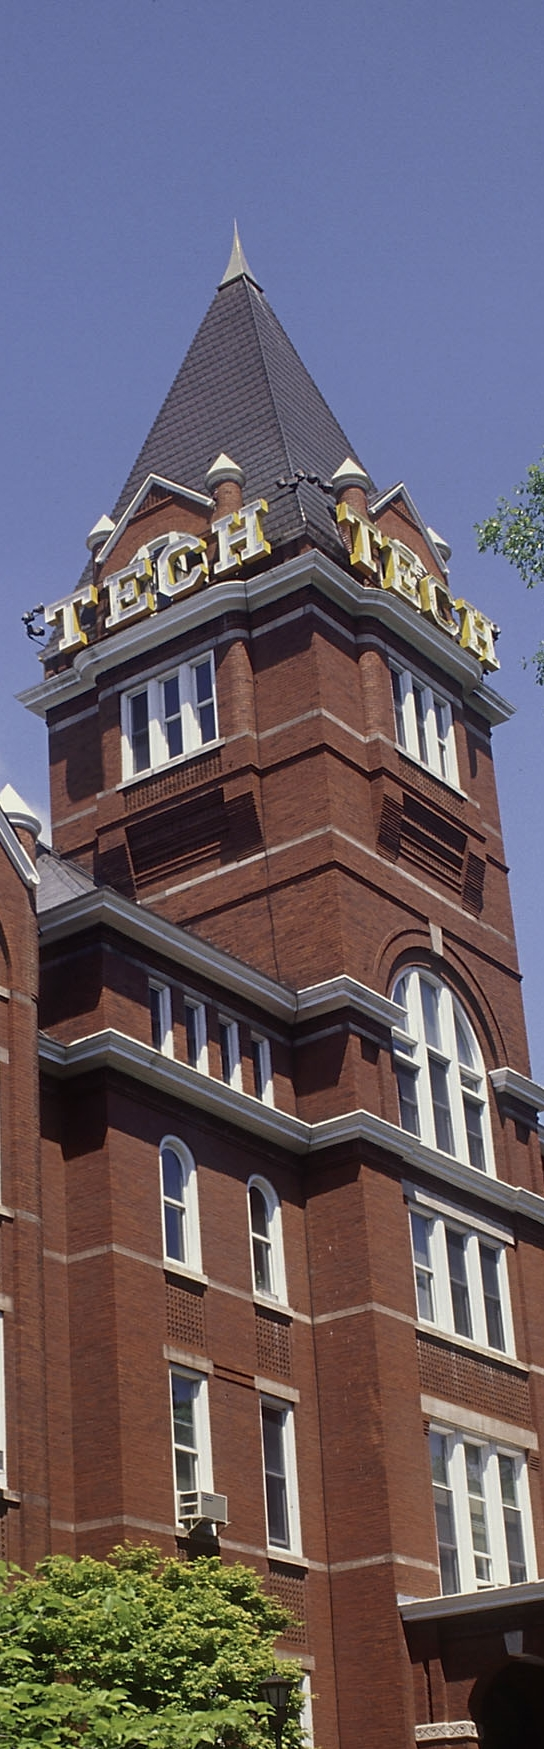
\includegraphics[width=1.25in]{figs/logo_TechTower.jpg}
    	\end{textblock}
    }

%logo tree
    \newcommand{\logoTree}
    {
    	\begin{textblock}{1}(0,0) 
    		\includegraphics[width=1.25in]{figs/logo_tree.jpg}
    	\end{textblock}
    }
%page numbers
    \newcommand{\mypagenum}
    {
    	\begin{textblock}{1}(1,94) 
		{\tiny \color[rgb]{0.2,0.2,1}\insertframenumber} %\insertframenumber,\insertpresentationendpage, \inserttotalframenumber
    	\end{textblock}
    }
%my footnote citation
	\newcommand{\myFootnoteCitation}[2]
	{
		\footnote{\tiny \citeauthor{#1}, \emph{#2}, \citeyear{#1}.}  %\citeauthor{#1}, \citetitle{#1}, #2 \citeyear{#1}.
	}
%my refer to citation
	\newcommand{\mycite}[1]
	{
		\emph{\citeauthor{#1} (\citeyear{#1})}
	}
%my footnote website citation
	\newcommand{\myFootnoteWebsiteCitation}[1]
	{
		\footnote{\tiny \citeauthor{#1}}
	}

\let\thefootnote\relax\footnotetext{Footnotetext without footnote mark}


%section underline
%\newcommand{\tmpsection}[1]{}
%\let\tmpsection=\section
%\renewcommand{\section}[1]{\tmpsection{\underline{#1}}}



%commands
	\newcommand{\likelihood}{p(Z_k| x_k) }						%likelihood
	\newcommand{\prior}{p(x_k)  } 								%prior
	\newcommand{\posterior} {p(x_k| Z_k)}						%posterior
	\newcommand{\prediction} {p(x_k| Z_{k-1})}					%prediction
	\newcommand{\update} {p(x_k|Z_k)}							%update
	\newcommand{\observations} {p(Z_k)}						%observations
	\newcommand{\prevobservations} {p(Z_{k-1})}				%previous observations
	\newcommand{\dxpk} {dx_{k-1}}							%dx_{k-1}
	\newcommand{\ChapKolm}{\int{p(x_k| x_{k-1})p(x_{k-1}|Z_{k-1})} \dxpk} %Chapman Kolmogorov

	%algorithm specific: JPDAF
	\newcommand{\likelihoodJPDAF}{p(Z_k| \chi, m, Z_{k-1}) }		%1. likelihood
	\newcommand{\priorJPDAF}{p(\chi|m, Z^{k-1}} 				%2. prior	
	\newcommand{\observationsJPDAF} {p(Z_k}					%3. observations
	\newcommand{\posteriorJPDAF} {p(\chi| Z_k)}					%4. posterior

%environments
	\newenvironment{changemargin}[2]
	{
	  	\begin{list}{}
		{
			\setlength{\topsep}{0pt}%
			\setlength{\leftmargin}{#1}%
			\setlength{\rightmargin}{#2}%
			\setlength{\listparindent}{\parindent}%
			\setlength{\itemindent}{\parindent}%
			\setlength{\parsep}{\parskip}%
		}
	  	\item[]
		}
		{\end{list}
	}
%figures

%colors
\definecolor{darkgreen}{rgb}{0,0.5,0}

%personal details
	\author{Salman Aslam}
	\institute{Advisor, Dr Christopher Barnes (ECE)\\Co-advisor, Dr Aaron Bobick (CoC)\\Georgia Institute of Technology}
	\date{}

\begin{document}
%####################################################################################################
\title{Signal Processing}
%####################################################################################################
\begin{frame}[plain]\logoTechTower
	\titlepage
\end{frame}

\begin{frame}
\frametitle{Outline}
\logoCSIPCPL\logoTechTower
	\setcounter{tocdepth}{1}	
	\tableofcontents
\end{frame}


%#######################################################################
\section{Introduction}
%#######################################################################
\begin{frame}
\frametitle{Introduction}
\logoEvolution\mypagenum
\end{frame}

%#######################################################################
\section{Non-Bayesian estimation}
%#######################################################################
\begin{frame}
\frametitle{Non-Bayesian estimators}
\framesubtitle{overview}
\logoEvolution\mypagenum
	\begin{figure}				
		\includegraphics[width=1.0\textwidth]{figs/SP_statisticalSP_overview.pdf}
	\end{figure}	
\end{frame}



\begin{frame}
\frametitle{Non-Bayesian estimators}
\framesubtitle{notation}
\footnote {\small Steven M Kay, \emph{Fundamentals of Statistical Signal Processing: Estimation Theory}, Prentice Hall, 1993}
\logoEvolution\mypagenum
	\begin{figure}				
		\includegraphics[width=1.0\textwidth]{figs/SP_likelihood.jpg}
	\end{figure}	
	$p(x;\theta)$
	\begin{itemize}
		\item the PDF is parameterized by the unknown parameter $\theta$
		\item a family of PDFs, i.e. a class of PDFs where each one is different due to a different value of $\theta$
	\end{itemize}			
\end{frame}




\begin{frame}
\frametitle{Non-Bayesian estimators}
\framesubtitle{max likelihood estimation}
\logoEvolution\mypagenum
	\begin{enumerate}				
		\item write a formula for the distribution of the unknown parameter $\theta$ in terms of the unknown parameter $\theta$ and the data $x$
			\begin{itemize}
				\item this is the {\color{blue}likelihood function}, formally defined as "the PDF viewed as a function of the unknown parameter $\theta$ and with the data $x$ fixed"
			\end{itemize}
		\item maximize it wrt $\theta$
			\begin{itemize}
				\item maximization is performed over allowable range of $\theta$
			\end{itemize}
		\item when closed form not available, numerical methods such as
			\begin{itemize}
				\item grid search
				\item iterative: Newton Raphson, scoring, EM
			\end{itemize}
	\end{enumerate}	
\end{frame}


%#######################################################################
\section{Distributions}
%#######################################################################
\begin{frame}[plain]
\frametitle{Common distributions (Duda \& Hart)}
\mypagenum
	\begin{changemargin}{-1.3in}{0in}
		\begin{figure}				
			\includegraphics[height=0.9\textheight]{figs/PRML_distributions_DudaHart.pdf}
		\end{figure}
	\end{changemargin}
\end{frame}


\begin{frame}
\frametitle{2D gaussian}
\logoEvolution\mypagenum
	\begin{figure}				
		\includegraphics[height=0.8\textheight]{figs/PRML_2D_gaussian.pdf}
	\end{figure}
\end{frame}


\begin{frame}
\frametitle{Poisson}
\logoEvolution\mypagenum
	\begin{figure}				
		\includegraphics[height=0.5\textheight]{figs/PRML_distributions_poisson.png}
	\end{figure}
\end{frame}



\begin{frame}
\frametitle{Binomial}
\logoEvolution\mypagenum
	Probability of getting k successes in n trials, where the probability of a single success is $p$
	\begin{itemize}
		\item In n trials, the number of {\color{red}ways} you can have k successes is
			\begin{equation*}
				\left(
				\begin{array}{c}
					 n \\ k	
				\end{array}
				\right)
				=
				\frac{n!}{(n-k)!k!}			
			\end{equation*}
		\item The probability of getting each of those {\color{red}ways} is
			\begin{equation*}
				p^k(1-p)^{n-k}
			\end{equation*}
		\item So, the total probability of getting k successes is 
			\begin{equation*}
				\text{bin}(k|n,p) =
				\left(
					\begin{array}{c}
						 n \\ k	
					\end{array}
				\right)
				p^k(1-p)^{n-k}
			\end{equation*}
		\item So, considering that $n$ and $p$ fixed, we can draw a plot between $k$ on the x-axis and bin$(k|n,p)$ on the y-axis
	\end{itemize}
\end{frame}



\begin{frame}
\frametitle{Binomial (cont.)}
\logoEvolution\mypagenum
	E$[k] = np$, VAR$[k]=np(1-p)$
\end{frame}



\begin{frame}
\frametitle{Signal to noise ratio}
\logoEvolution\mypagenum
	\begin{itemize}
		\item Signal power,
			\begin{align*}
				\sigma^2 	&= E\left[(x-\mu_x^2) \right] \\
							&= \int\limits_{-\infty}^{\infty} (x-\mu_x)^2 f_X(x)dx
			\end{align*}
	\end{itemize}
\end{frame}


%#######################################################################
\section{Definitions}
%#######################################################################

%=================================================================
\subsection{Covariance Matrix}
%=================================================================
\begin{frame}
\frametitle{Covariance matrix}
\logoEvolution\mypagenum
	We have a signal with a $n$ random variables, $X_1, X_2, ... X_n$.  To find the covariance matrix,
	\begin{enumerate}
		\item Take one realization, as shown in the next figure.
		\item For this realization, multiply $X_1$ with $X_1$, $X_1$ with $X_2$, $X_1$ with $X_n$, and so on.
		\item Now take many more realizations and find the average values of the multiplications above.
		\item Now fill the covariance matrix, $VAR[X_1] = E[X_1X_1]$
	\end{enumerate}
\end{frame}




\begin{frame}
\frametitle{Covariance matrix (cont.)}
\logoEvolution\mypagenum
	We assume zero mean random variables.  If they're not, just subtract the mean.	
	\begin{figure}
		\centering
		\includegraphics[width=1.0\textwidth]{figs/SP_covariance.pdf}
		\label{fig:Covariance}
	\end{figure}
\end{frame}



\begin{frame}\frametitle{Covariance matrix (cont.)}\logoEvolution\mypagenum
	Again, assume zero mean random variables.
	\begin{figure}
		\includegraphics[height=0.9\textwidth]{figs/SP_covariance_example.pdf}
	\end{figure}
\end{frame}



%%=================================================================
%\subsection{Stationarity}
%%=================================================================
%\begin{frame}
%\frametitle{Stationarity}
%\logoEvolution\mypagenum
%	\begin{itemize}
%		\item Random process $X(t)$
%		\item Take its samples $X(t_1), X(t_2), X(t_3), ...X(t_k)$
%		\begin{equation*}
%			p_{X(t_1), X(t_2), \ldots X(t_k)}= p_{X(t_{1+\tau}), X(t_{2+\tau}), \ldots X(t_{k+\tau})}
%		\end{equation*}
%		$\forall t, k, \tau$ 
%	\end{itemize}
%\end{frame}


%=================================================================
\subsection{Ergodicity}
%=================================================================
\begin{frame}
\frametitle{Ergodicity}
\logoEvolution\mypagenum
	\begin{itemize}
		\item Random process $X(t)$
		\item Take its samples $X(t_1), X(t_2), X(t_3), ...X(t_k)$
		\begin{equation*}
			p_{X(t_1), X(t_2), \ldots X(t_k)}= p_{X(t_{1+\tau}), X(t_{2+\tau}), \ldots X(t_{k+\tau})}
		\end{equation*}
	\end{itemize}
\end{frame}


%=================================================================
\subsection{Laws of Large Numbers}
%=================================================================
\begin{frame}
\frametitle{Weak Law of Large Numbers}
\logoEvolution\mypagenum
	\begin{itemize}
		\item $X_0, X_1, \ldots, X_{N-1}$ is a sequence of i.i.d. random variables
		\item  $E[X]=\mu$
		\item for $\epsilon > 0$
			\begin{equation*}
				\lim_{n\rightarrow \infty} P[(M_n-\mu)<\epsilon]=1
			\end{equation*}
			where,
			\begin{equation*}
				M_n=\frac{1}{N}\sum\limits_{n=0}^{N-1}X_n
			\end{equation*} 
	\end{itemize}
\end{frame}


%=================================================================
\subsection{Correlation}
%=================================================================
\begin{frame}
\frametitle{Weak Law of Large Numbers}
\logoEvolution\mypagenum
	\begin{itemize}
		\item Take 2 random variables $X$ and $Y$ centered around 0, i.e., $E[X]=0, E[Y]=0$, we want to know what is $E[XY]$
		\begin{equation*}
		a
		\end{equation*}
	\end{itemize}
\end{frame}


%#######################################################################
\end{document}
%#######################################################################